\label{sec:approach}

Two commonly used retrieval models are Boolean Model (also Extended Boolean model), and
Vector Space Model. Both have some strong sides as well as some weak sides. We need to pick
the most appropriate one.

\subsection{Boolean Model}
\label{sec:boolean}
Boolean model [2] depends on set operation. Documents are represented as a set of keywords.
User queries are expressed as Boolean expression of keywords connected by AND, OR, and
NOT while brackets are used to indicate scope. For example a query is like below:

\textit{(Text \textbf{OR} information) \textbf{AND} Retrieval \textbf{AND} (\textbf{NOT}) Theory}

A document containing \texttt{text information retrieval} or \texttt{text retrieval} will be a match. On the
other hand texttt{information retrieval theory} will not be present in search result because of having
texttt{theory} in document. Boolean Model's positive sides are, it is easy to understand for simple
queries and for normal user queries it is easy to implement. On the other hand, it has lots of
limitations:
\begin{itemize}
\item \textbf{Firstly},  it is very rigid where AND means all, OR means any. So it returns either too many search results or too few.
\item \textbf{Secondly}, it is difficult to express complex user queries for peoples
with limited knowledge about set operation.
\item \textbf{Thridly},  it is difficult to incorporate relevance feedback via query modification
\item \textbf{Fourthly}, Basic Boolean Model does not support to order the search result according to the relevance score with search query. However, Boolean Model can be extended to support this ranking [3]. Given the limitation of Boolean Model we need to pick some model which can distinguish important words in a document for weighted comparison. We need a similarity measure between document and user query
\item \textbf{Lastly}, we need a way to incorporate relevance feedback of user via
query modification. This leads to Vector Space Model(Section~\ref{sssec:vsm-desc}).
\end{itemize}

\begin{figure}
\center
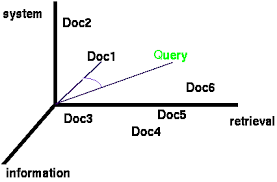
\includegraphics[width=0.5\linewidth]{figures/vsm}
\label{fig:vsm}
\caption{Vector Space Model}
\end{figure}

\subsection{Vector Space Model}
\label{sec:vsm-desc}
Vector Space Model [4] is also known as Term Vector Model. It is an algebraic model for
representing text documents as vectors of terms where a weight is associated with each term
dimension. User query on the other hand is also represented as a vector of terms. A similarity
score like, Euclidian Distance, Manhattan Distance, Inner Product, or Cosine can be used to
measure the similarity score between document vector and query vector. Figure 1 depicts an
example of Vector Space Model. Strength of Vector Space Model are:

\begin{itemize}
\item It is simple and mathematically based model.
\item It takes into account both local importance in a document and global importance in the whole corpus.
\item It provides partial matching with query and ranked result.
\item It works quite well practically.
\item It is possible to have an efficient implementation of this algorithm to provide a fast ranking of relevant documents.
\end{itemize}
Despite all the strong factors it has some limitations too.
\begin{itemize}
\item It does to take into account the
semantic meaning of words, or their occurrence orders.
\item We lack the control of rigidly returning search results.
\end{itemize}
Despite these weaknesses there many strong factors of Vector Space Model and that’s why we have selected it as our retrieval model.
